Рассмотрим работу алгоритмов на матрицах стоимостей размера $N \times N$.

\section{Алгоритм полного перебора}
\qquadСначала составляются все возможные маршруты, проходящие через все города ровно по одному разу и возвращающиеся в начальный пункт.\\

Затем каждая такая перестановка анализируется на предмет существования, и, если такой маршрут можно проложить, то находится его длина с помощью матрицы стоимостей, если же нельзя, то проверяется следующий и т.д. \\

В случае, если полученное значение длины оказывается меньше текущего минимального, то и этот маршрут, и его длина запоминаются в качестве потенциального решения задачи, и дальнейшие сравнения будут проходить уже с этими величинами. Таким образом, просматриваются все возможные варианты маршрутов.\\

Схема алгоритма представлена на Рис.\ref{fig1:image}, \ref{fig2:image}.

\begin{figure}[h]
	\begin{center}
		{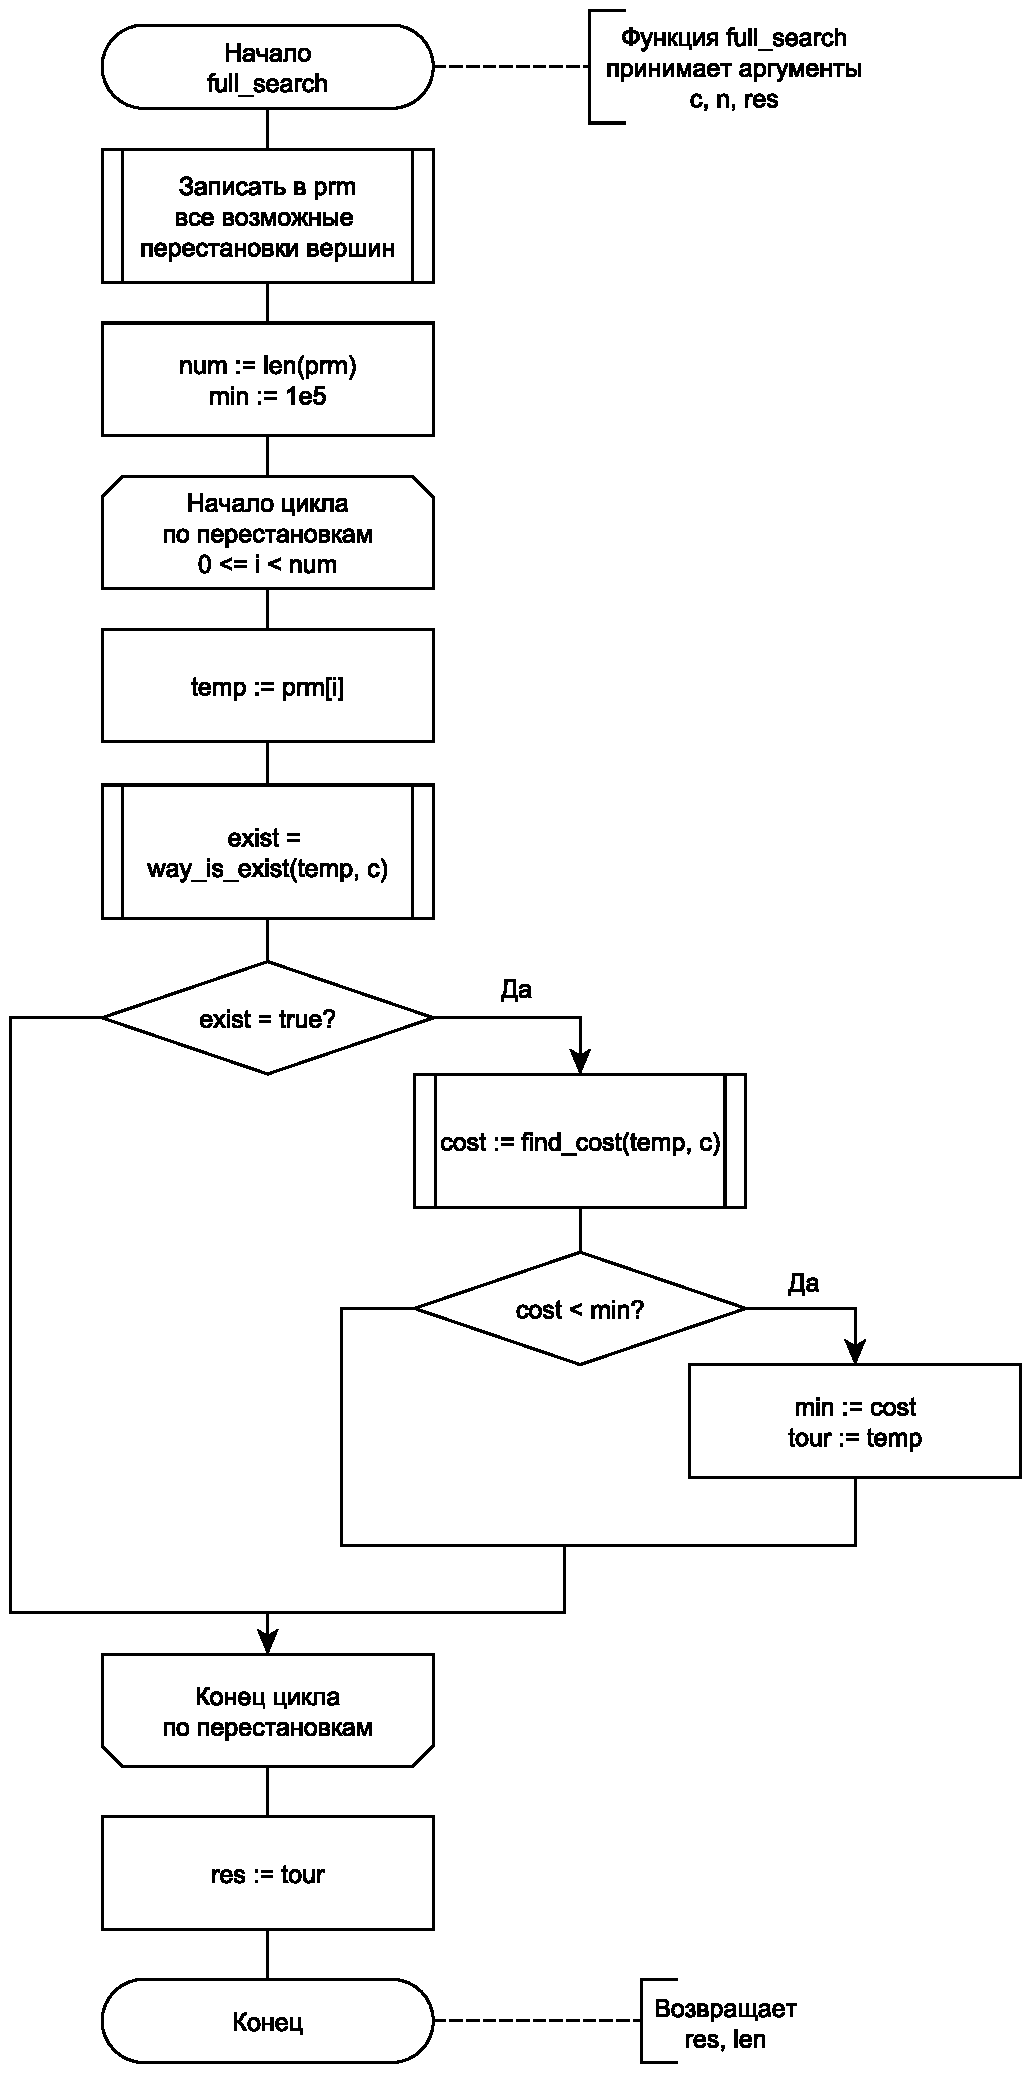
\includegraphics[scale = 0.6]{schemes/full}}
		\caption{Алгоритм полного перебора (часть 1)}
		\label{fig1:image}
	\end{center}
\end{figure}

\begin{figure}[h]
	\begin{center}
		{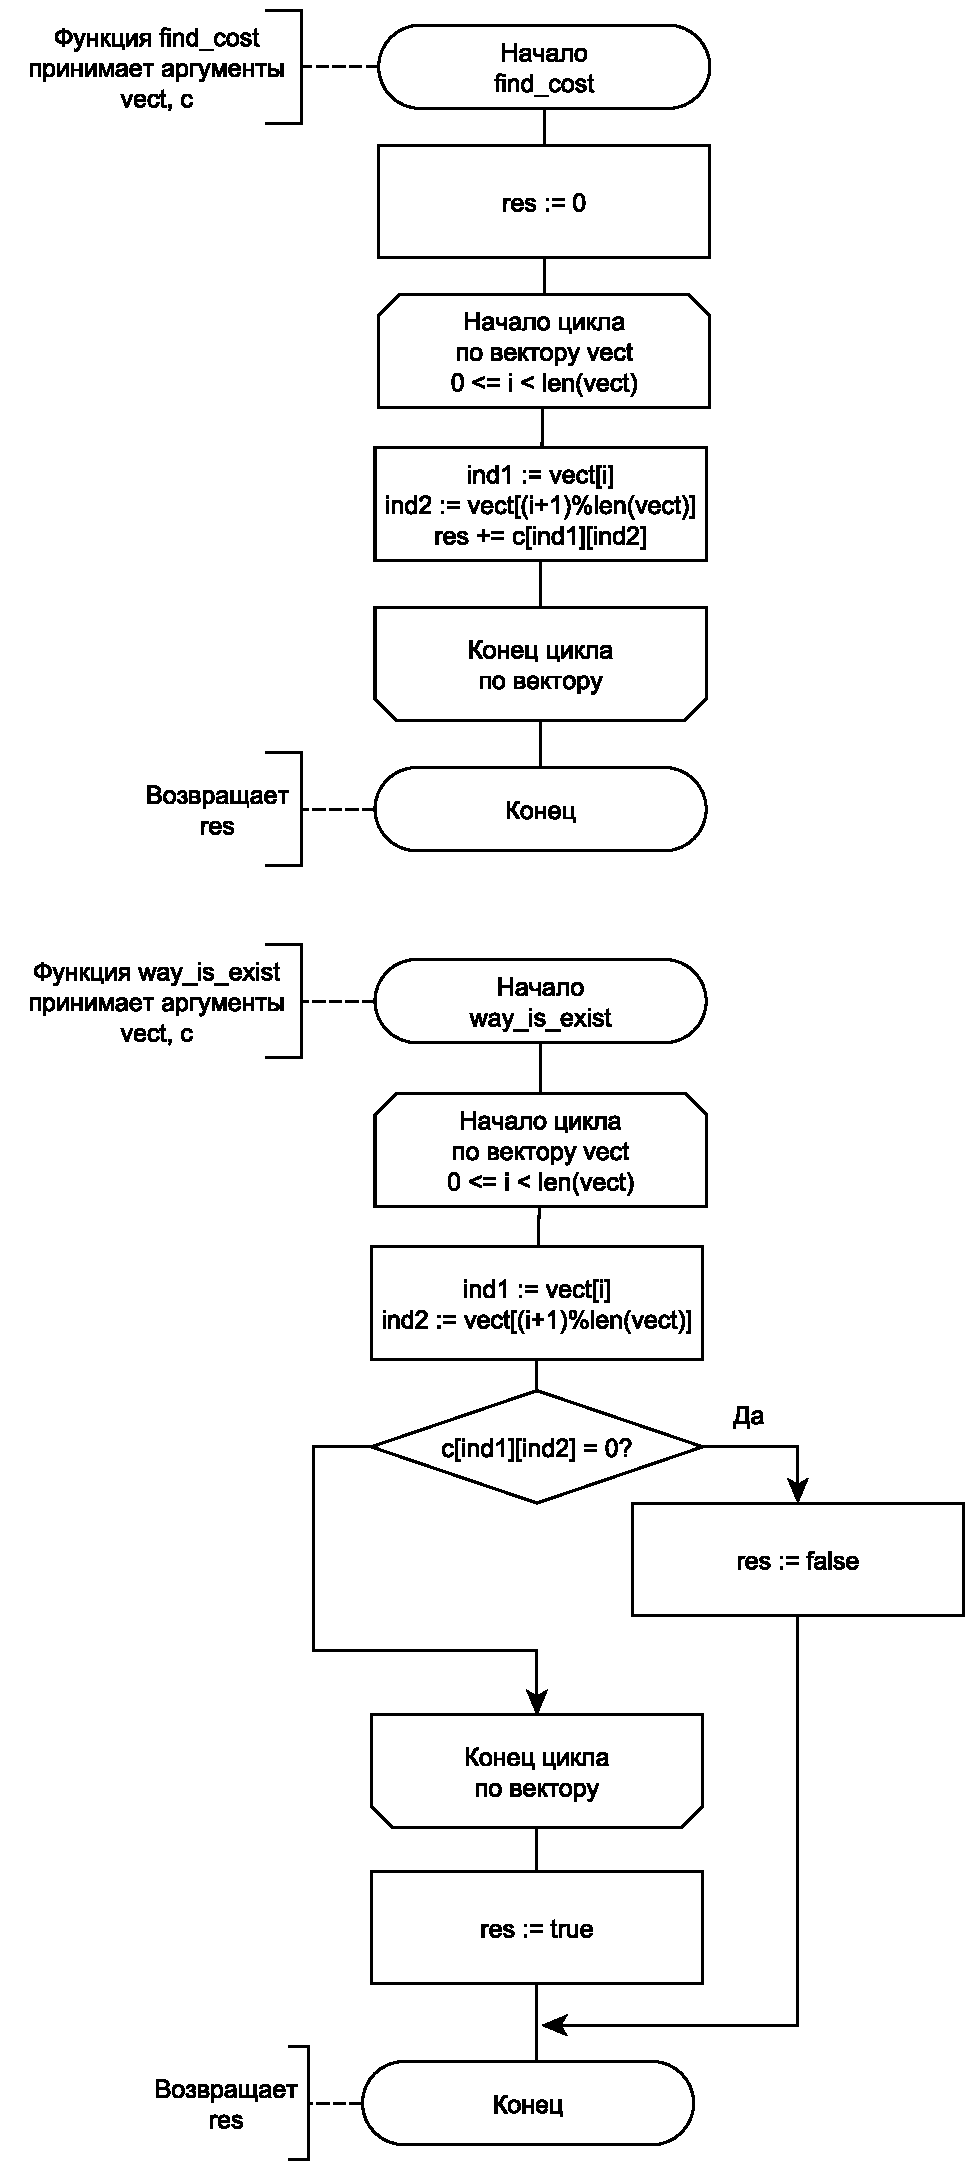
\includegraphics[scale = 0.6]{schemes/full2}}
		\caption{Алгоритм полного перебора (часть 2)}
		\label{fig2:image}
	\end{center}
\end{figure}

\section{Муравьиный алгоритм}
\qquadВ начале работы алгоритма задаются равные значения феромонов на каждой вершине.\\

Затем осуществляется проход по каждому из отведённых дней, создаётся колония из $N$ муравьёв, причём каждому муравью ставится в соответствие свой город, в качестве начальной позиции. Для каждой особи составляется список вершин, которые обязательно должны быть пройдены, и по мере передвижения уже посещённые будут из него удаляться. \\

Процесс построения маршрута будет продолжаться до тех пор, пока этот список не станет пустым, или, пока не произойдёт тупиковая ситуация, когда из вершины никуда дальше перейти нельзя.\\

Чтобы обеспечить выполнение условия замкнутости, дополнительно в список непосещённых вершин добавляется начальная, когда все остальные вершины успешно пройдены.\\

Для того, чтобы определить, через какой узел маршрут пройдёт дальше, алгоритм делает следующее: выполняет проход по списку непосещённых вершин и проверяет по таблице стоимостей, возможно ли перейти из текущей позиции в рассматриваемую. И, исходя из этого, применяются соответсвующие формулы рассчёта. В результате, будет либо выбрана какая-либо вершина, либо сделан вывод о том, что муравей попал в тупик. \\

По мере того, как прокладывается маршрут, данные о его длине и компонентах постоянно обновляются. \\

Если маршрут успешно построен, то сравнивается полученный результат с промежуточным ответом, последний обновляется, если первый оказывается меньшим по длине. Затем алгоритм учитывает испарение феромона, а также вклад <<элитных>> муравьёв, увеличивающих концентрацию феромона на минимальном по длине участке, и всей колонии в целом.\\

Выполнив все необходимые действия, алгоритм возвращает итоговый результат.\\

Схема алгоритма представлена на Рис.\ref{fig3:image}, \ref{fig4:image}, \ref{fig5:image}, \ref{fig6:image}, \ref{fig7:image}.

\begin{figure}[h]
	\begin{center}
		{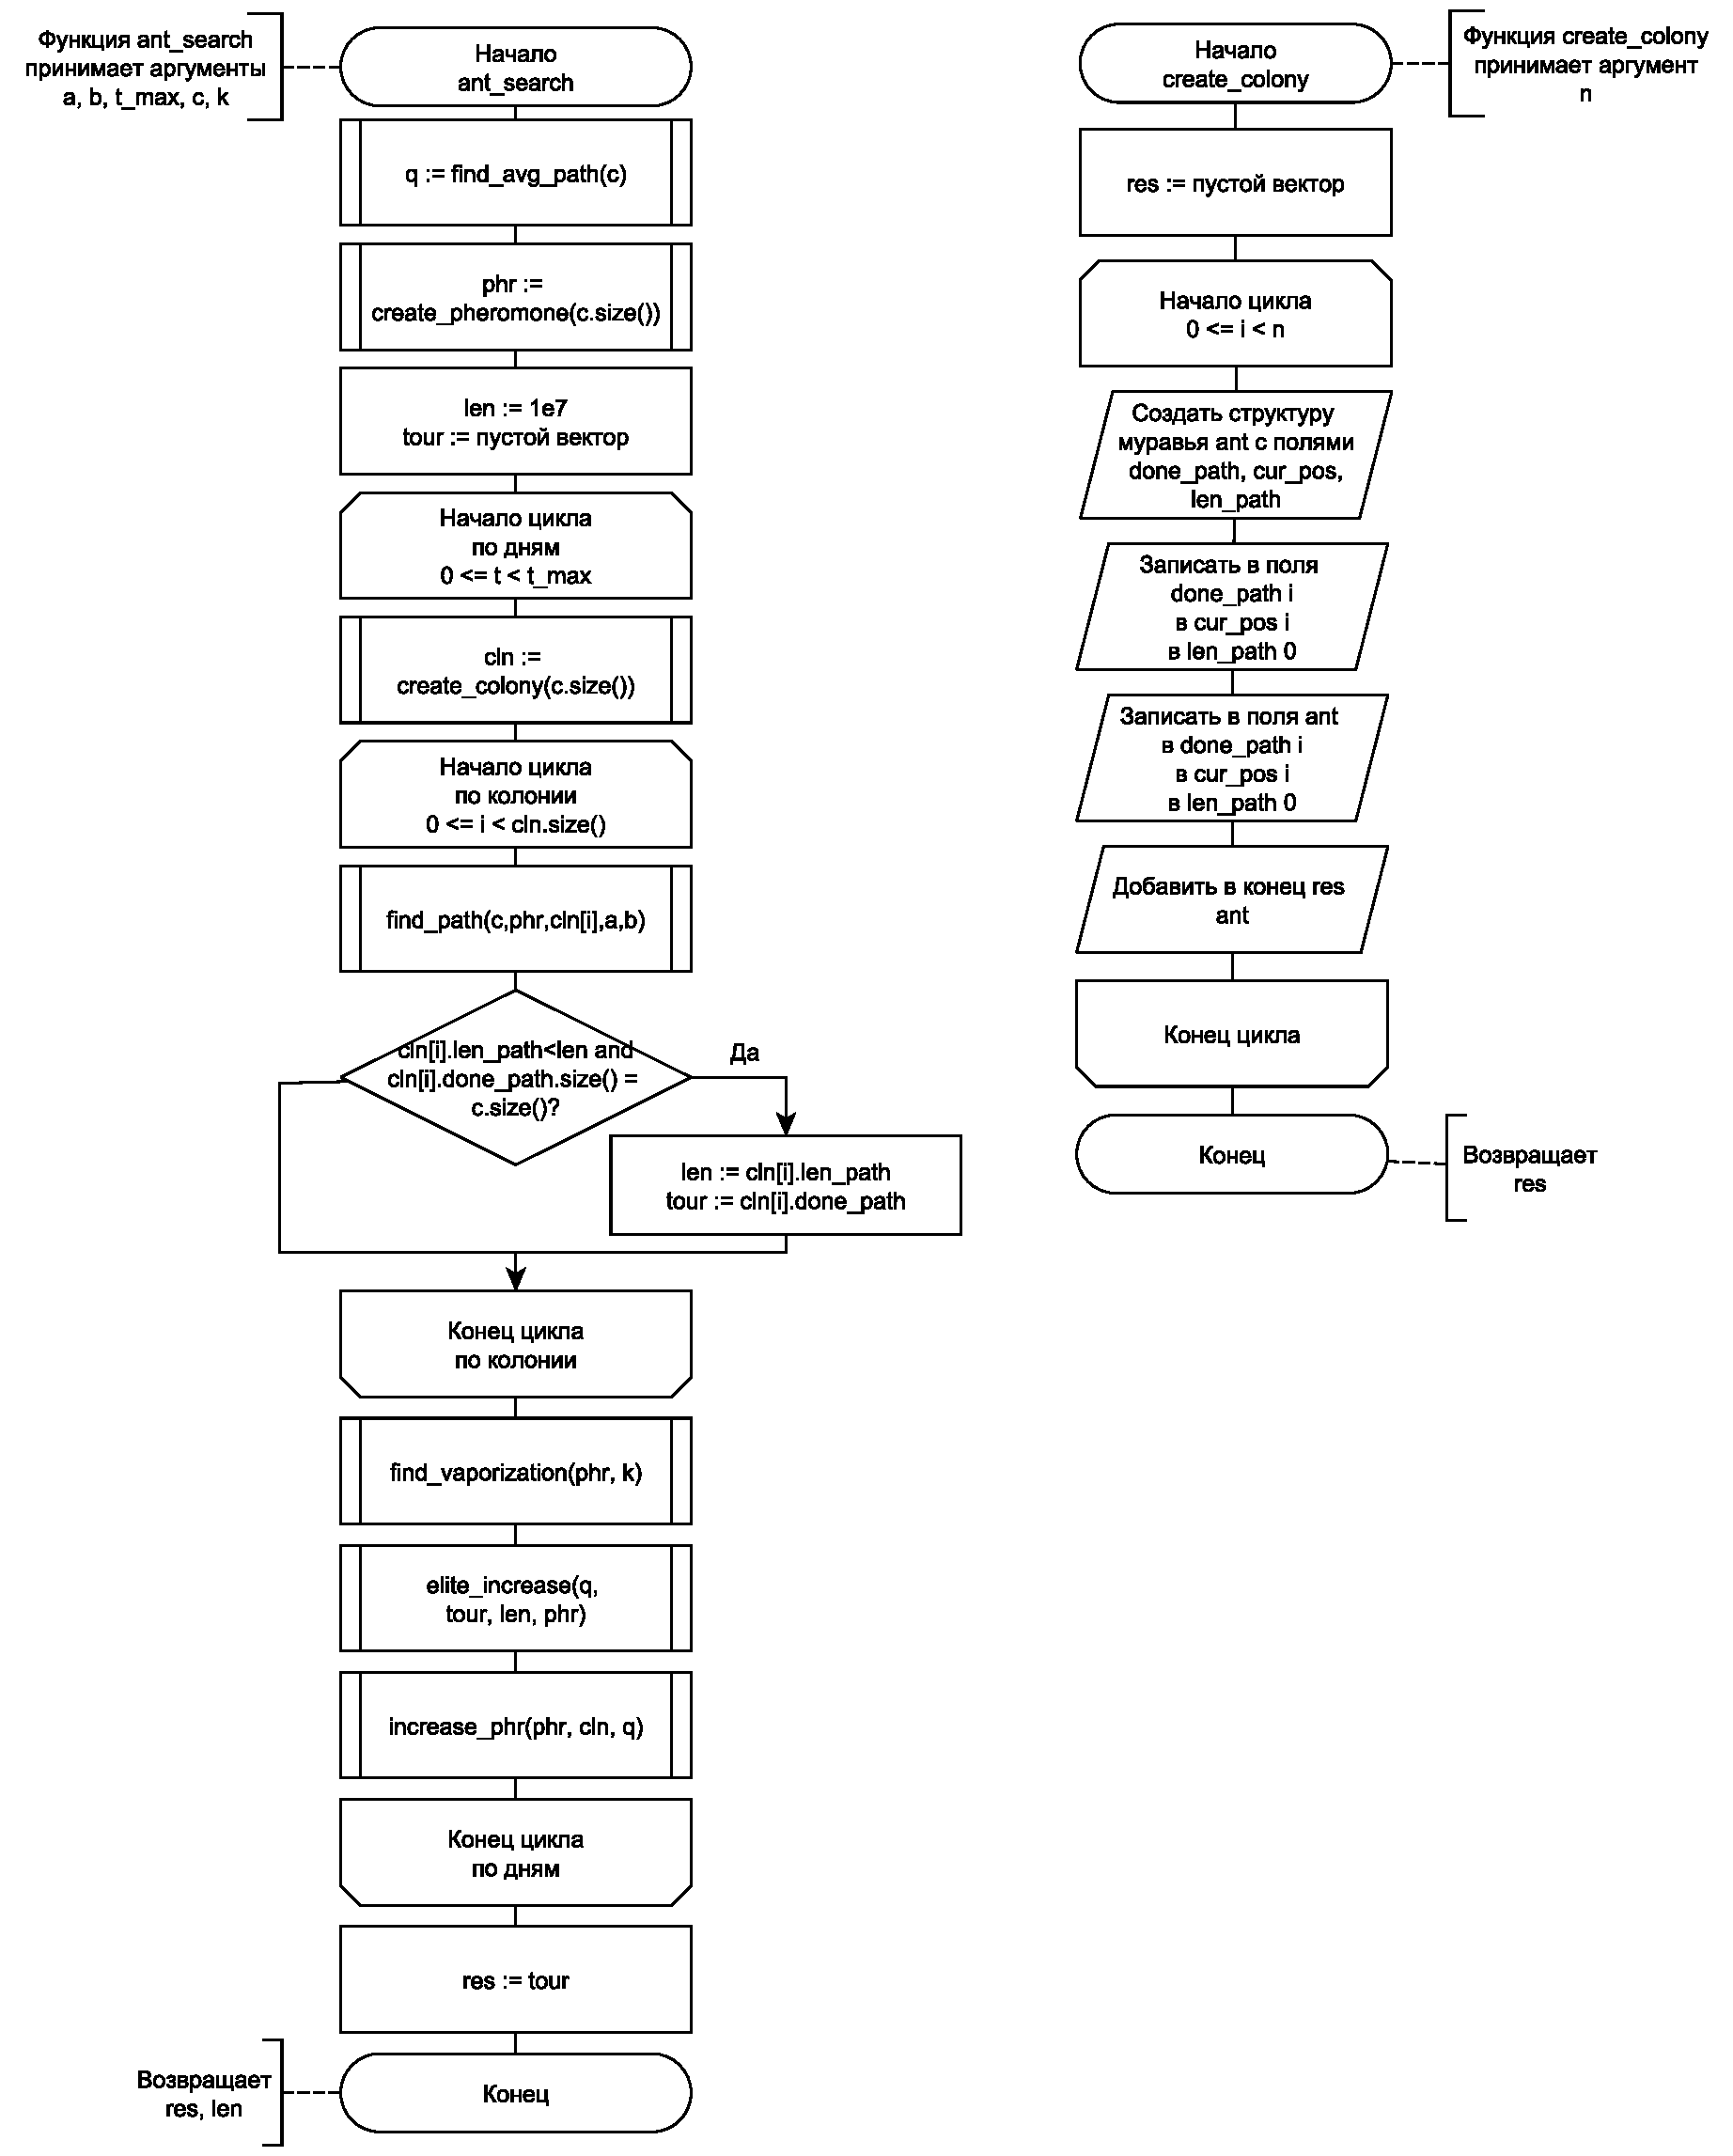
\includegraphics[scale = 0.6]{schemes/ant1}}
		\caption{Муравьиный алгоритм (часть 1)}
		\label{fig3:image}
	\end{center}
\end{figure}

\begin{figure}[h]
	\begin{center}
		{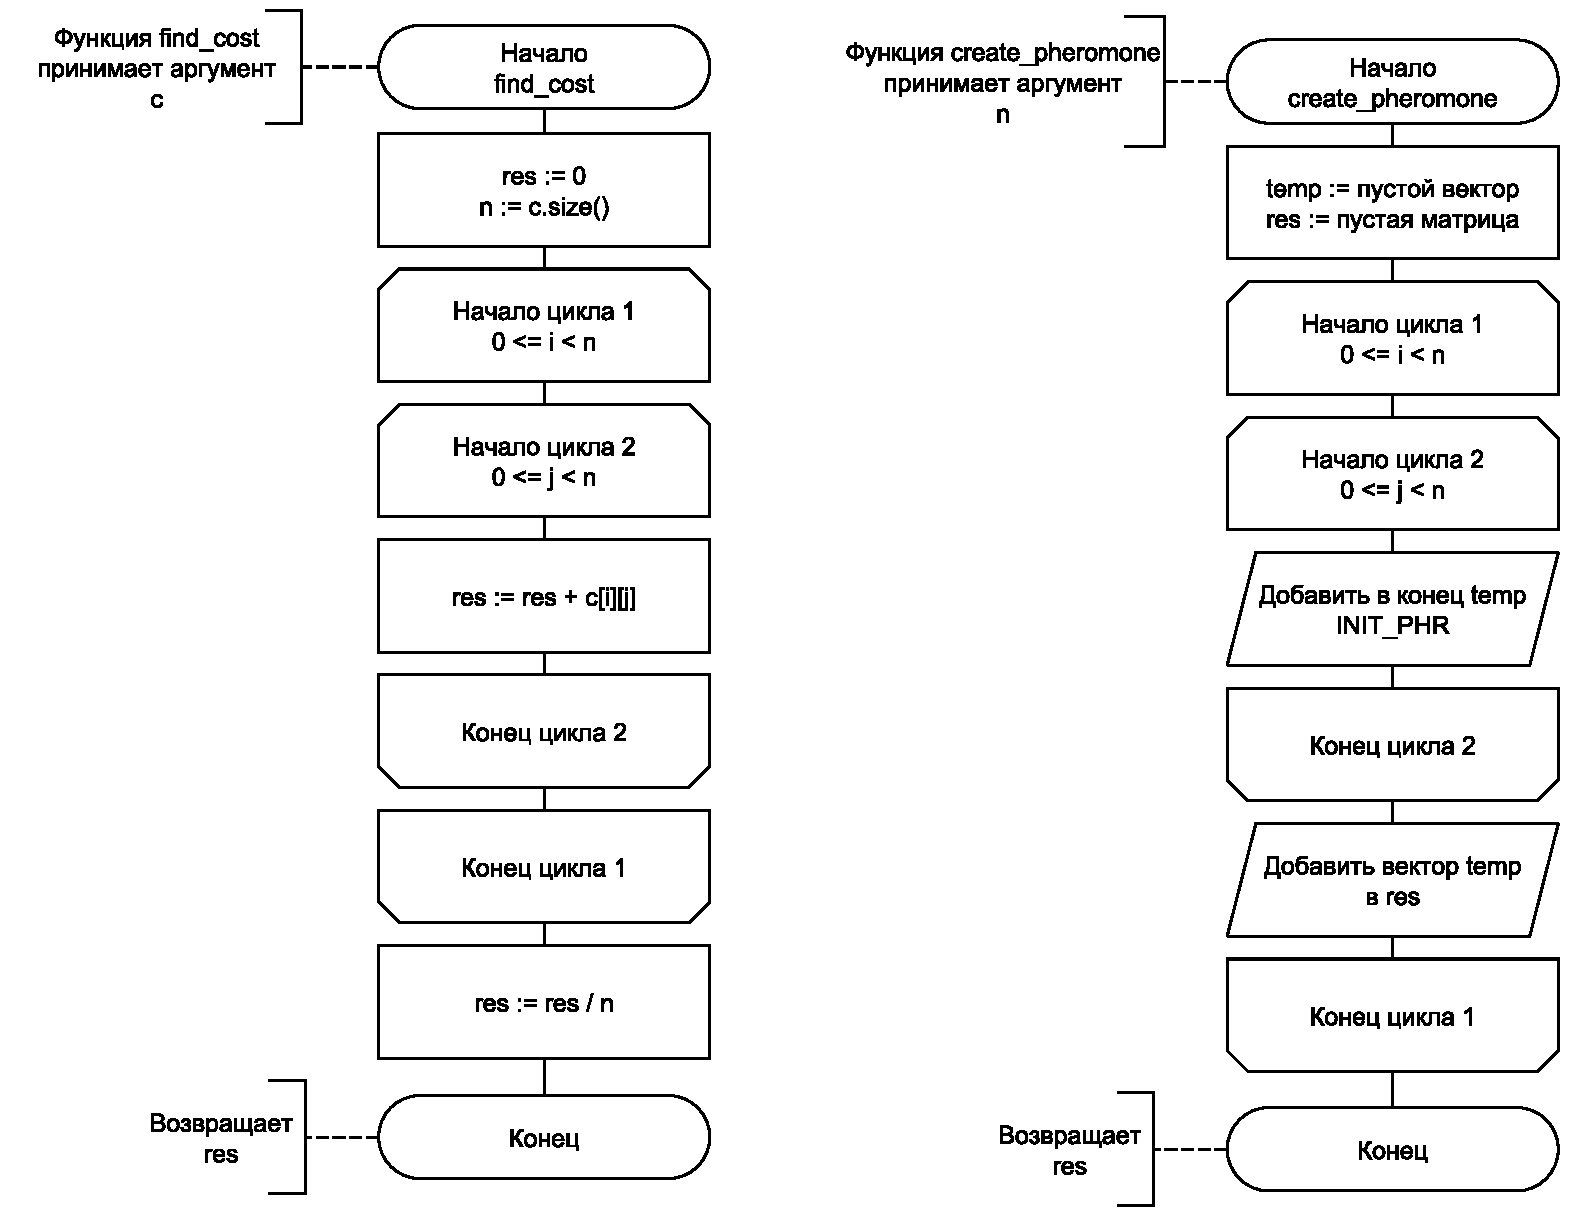
\includegraphics[scale = 0.6]{schemes/ant2}}
		\caption{Муравьиный алгоритм (часть 2)}
		\label{fig4:image}
	\end{center}
\end{figure}

\begin{figure}[h]
	\begin{center}
		{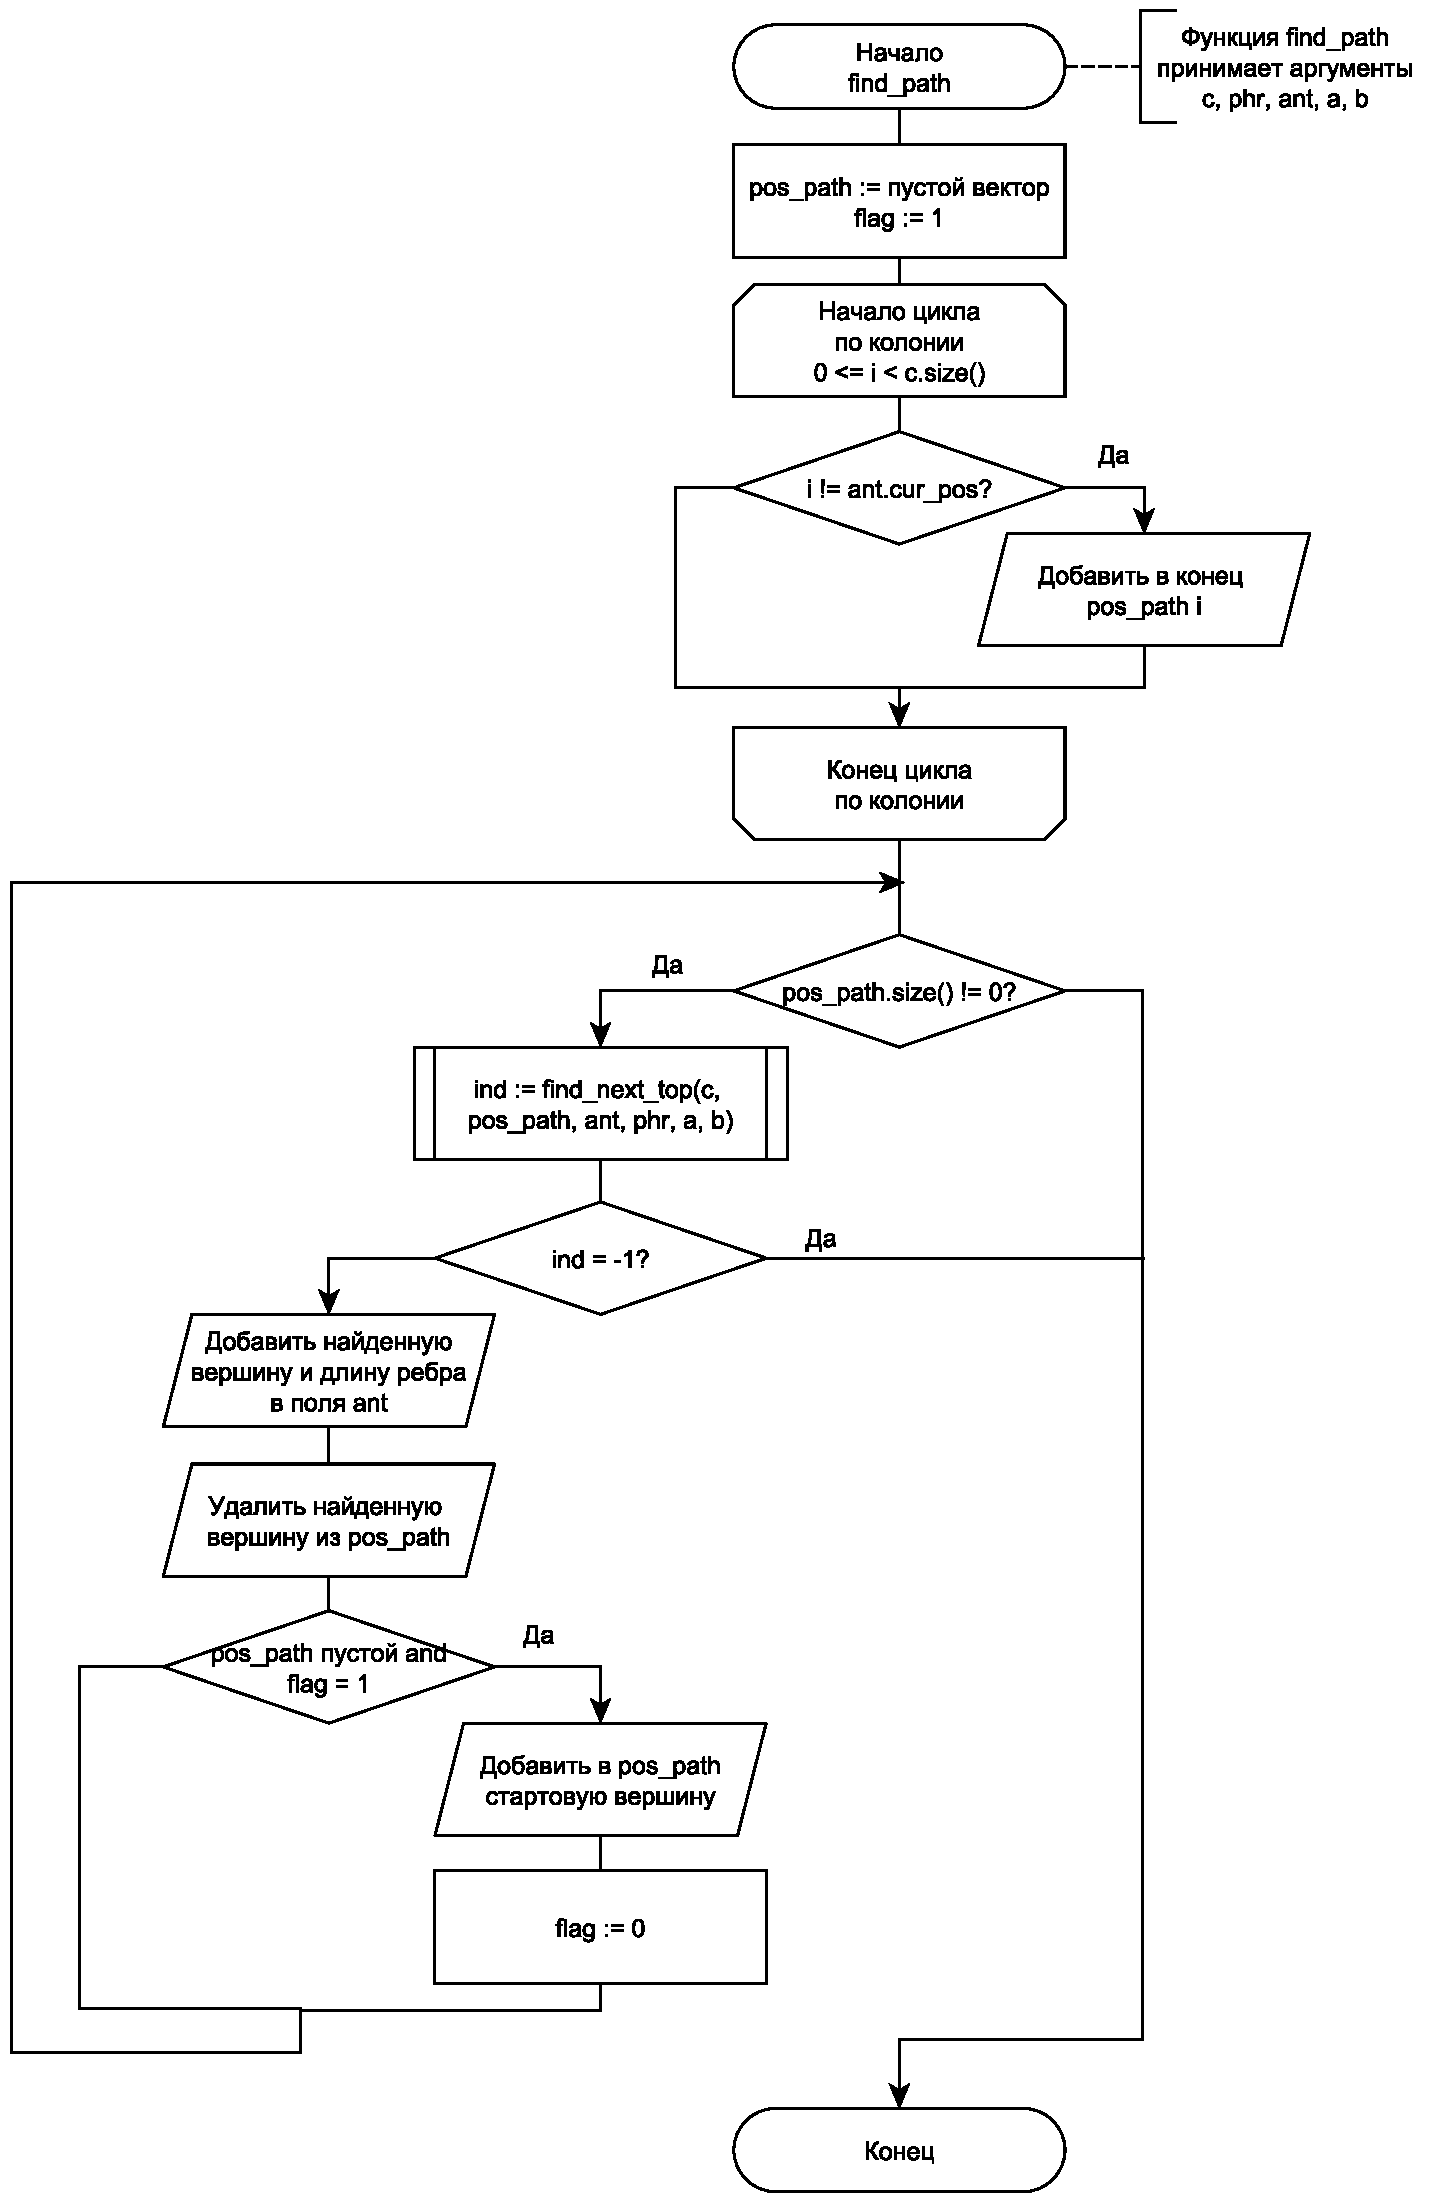
\includegraphics[scale = 0.6]{schemes/ant3}}
		\caption{Муравьиный алгоритм (часть 3)}
		\label{fig5:image}
	\end{center}
\end{figure}

\begin{figure}[h]
	\begin{center}
		{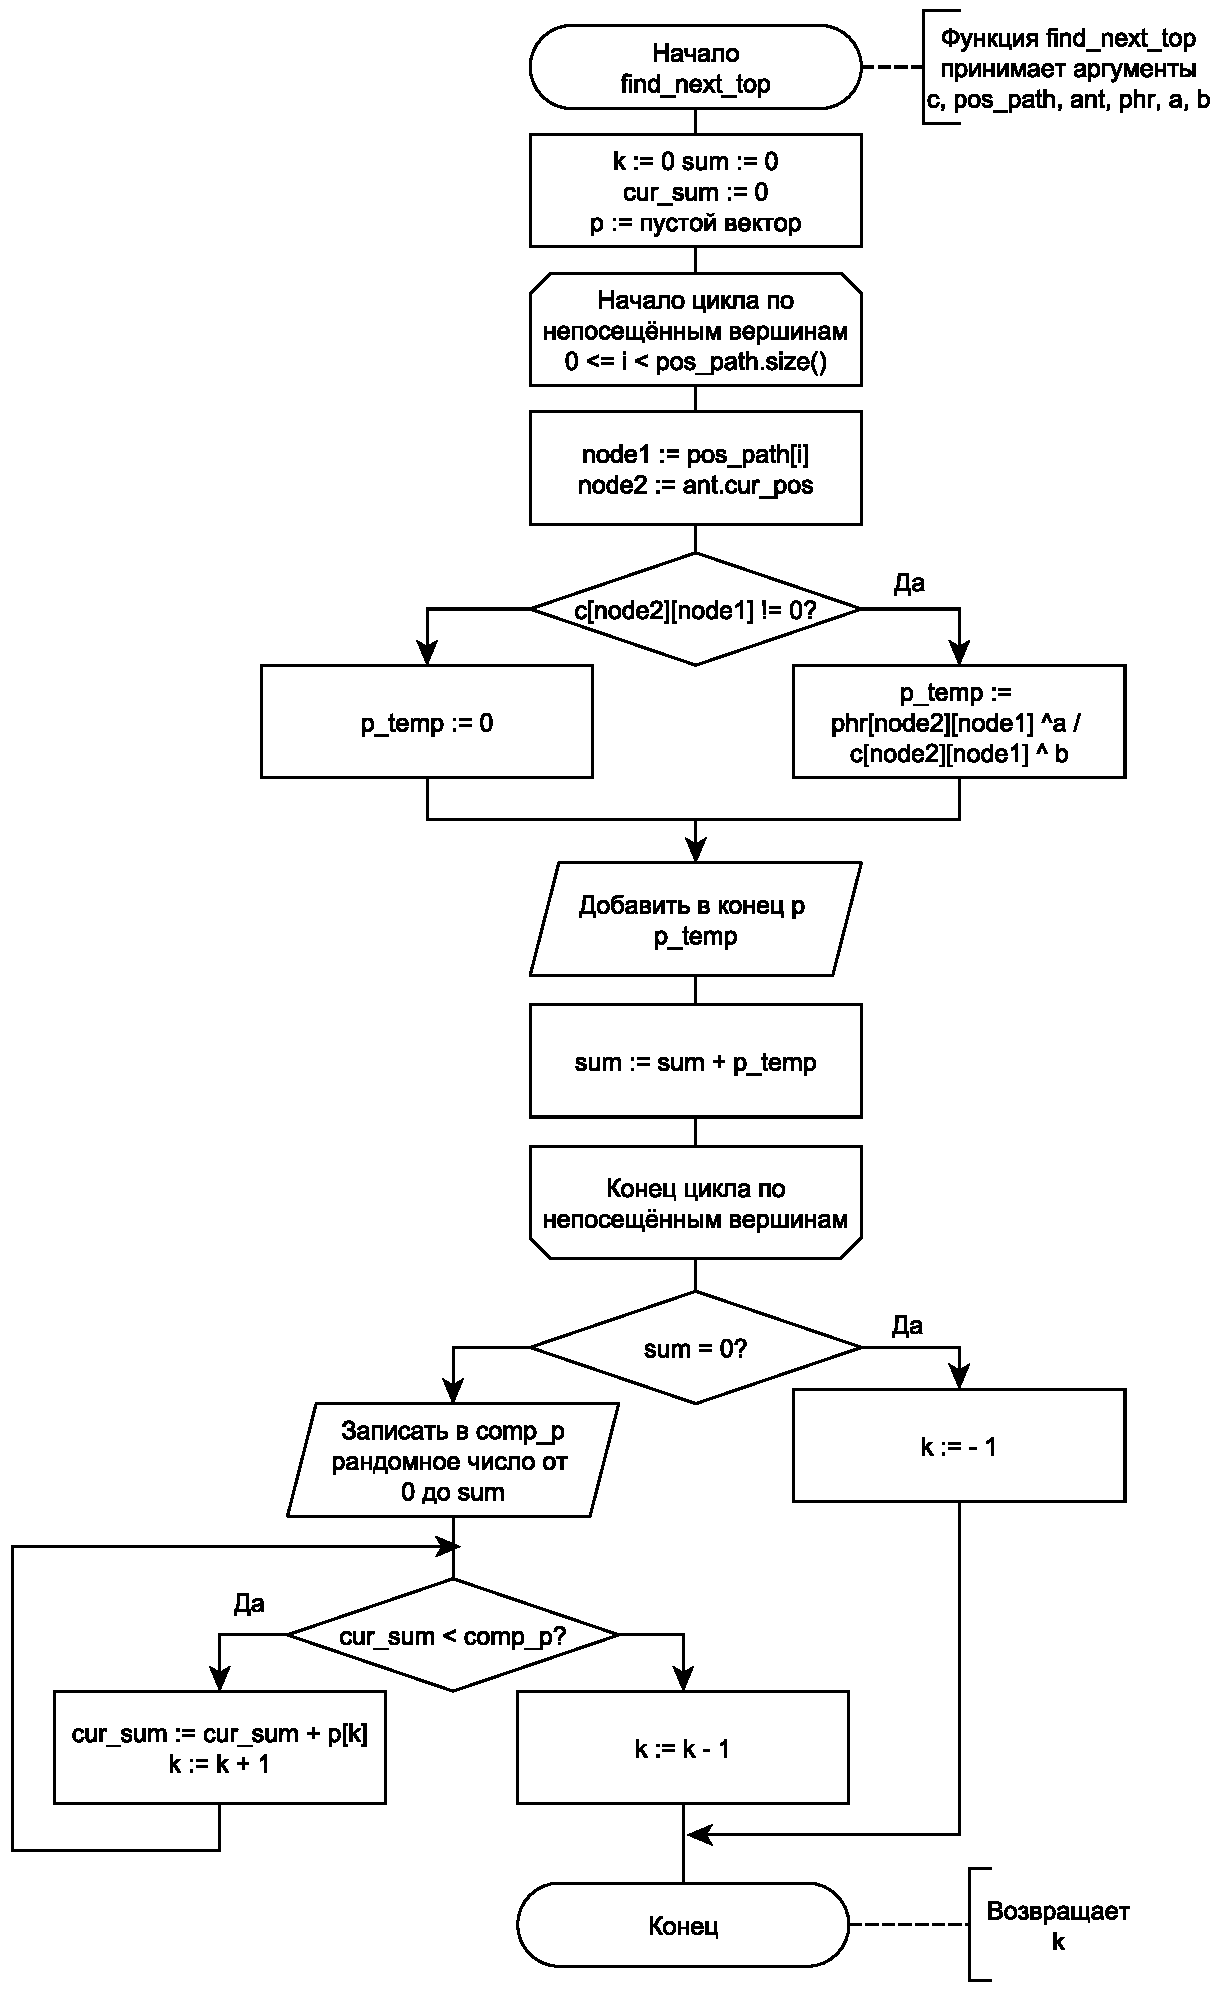
\includegraphics[scale = 0.6]{schemes/ant4}}
		\caption{Муравьиный алгоритм (часть 4)}
		\label{fig6:image}
	\end{center}
\end{figure}

\begin{figure}[h]
	\begin{center}
		{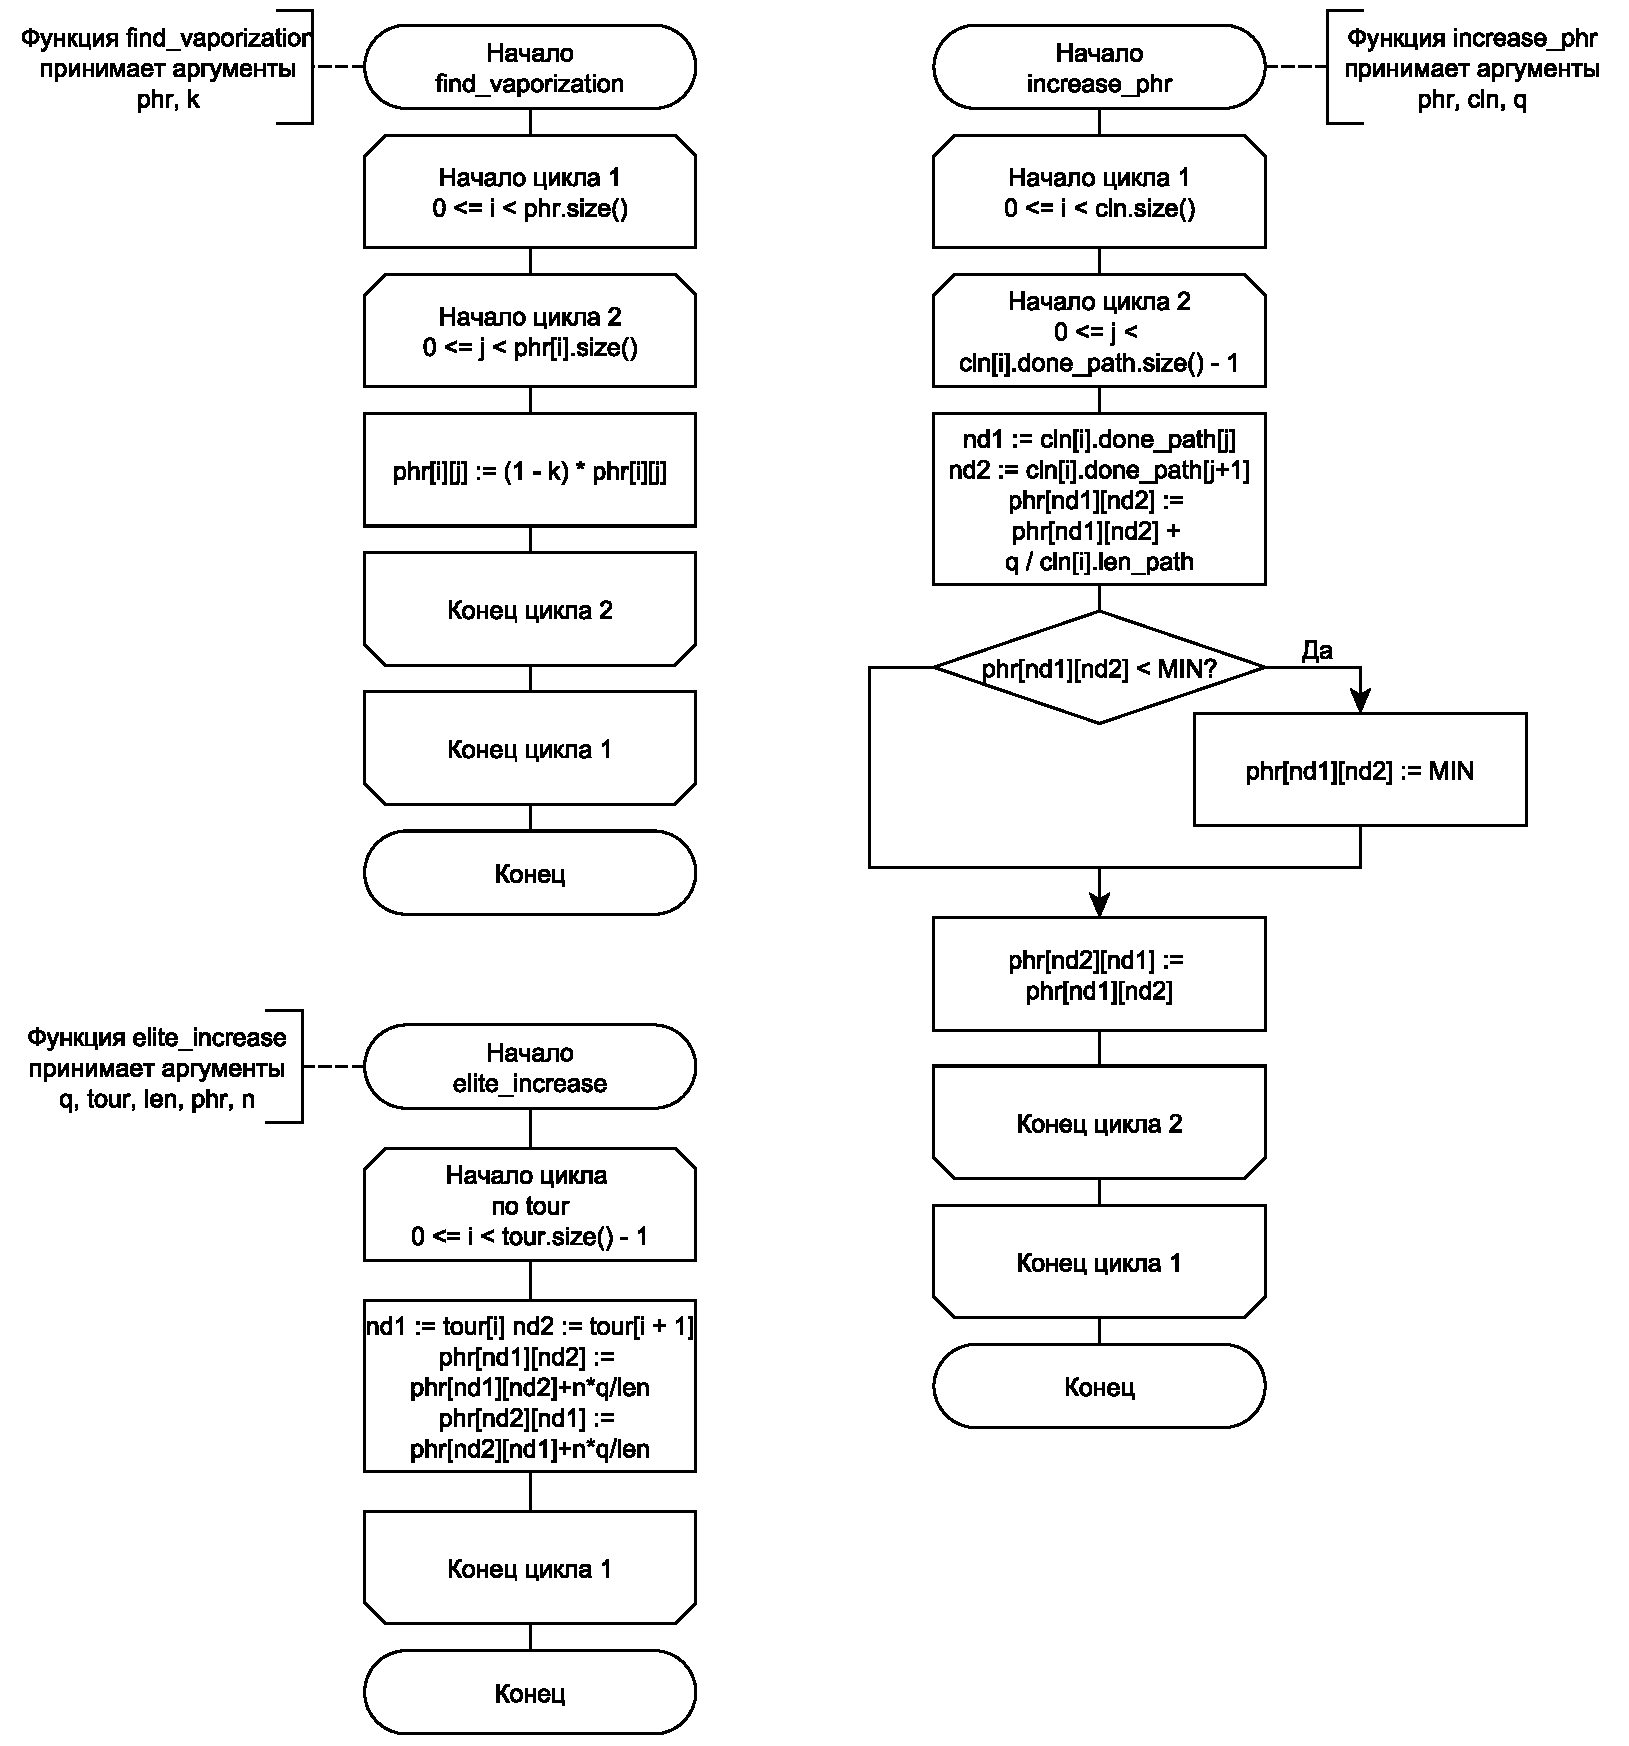
\includegraphics[scale = 0.6]{schemes/ant5}}
		\caption{Муравьиный алгоритм (часть 5)}
		\label{fig7:image}
	\end{center}
\end{figure}

\section{Автоматизация параметризации}
\qquadАвтоматизация параметризации проводится на базе муравьиного алгоритма, поскольку, как видно из формул \ref{formula2}, \ref{formula4}, результат сильно зависит от используемых параметров, которые различаются в зависимости от данных конкретной задачи. Поэтому, для поиска нужных значений нужно создать алгоритм, который бы перебирал их, выполнял поставленную задачу для каждого набора параметров и путём анализа выбирал тот, у которого наилучшие показатели.

\section{Требования к ПО}
\qquadДля корректной работы алгоритмов и проведения тестов необходимо выполнить следующее.
\begin{itemize}
	\item Обеспечить возможность ввода количества городов и выбора алгоритма через консоль.
	\item В случае ввода некорректных данных вывести соответствующее сообщение. Программа не должна аварийно завершаться.
	\item Реализовать функцию, осуществляющую испытания муравьиного алгоритмами с различными значениями параметров, вывести результаты на экран.
\end{itemize}

\section{Заготовки тестов}
\qquadПри проверке на корректность работы необходимо провести следующие тесты:
\begin{itemize}
	\item стандартный тест;
	\item число городов $N$ = 2;
	\item нет решения;
	\item два или более маршрута с одинаковой протяженностью.
\end{itemize}

\section*{Вывод}
\addcontentsline{toc}{section}{Вывод}
\qquadВ этом разделе разобраны основные принципы выбранных алгоритмов, приведены схемы работы каждого из них, сформулированы требования к программному обеспечению и сделаны заготовки тестов.




























